\documentclass[11pt,letter]{article}
\usepackage[top=1.00in, bottom=1.0in, left=1.1in, right=1.1in]{geometry}
\renewcommand{\baselinestretch}{1.1}
\usepackage{graphicx}
\usepackage{natbib}
\usepackage{amsmath}
\usepackage{xcolor}
\usepackage{color,soul} %to highlight text; just write \hl{highlighted text}
\usepackage{hyperref}

\def\labelitemi{--}
\parindent=0pt

\begin{document}
\bibliographystyle{/Users/Lizzie/Documents/EndnoteRelated/Bibtex/styles/besjournals}
\renewcommand{\refname}{\CHead{}}

\title{phenomenological and dynamical models for understanding long transients.}
\author{Arroyo-Esquivel, Boettiger, Jiang, Reimer, Scharf, Wolkovich, Zhu}
\date{\today}
\maketitle

%%%%%%%%%%%%%%%%%%%%%%%%%%%%%%%%%%%%%%%%%%%%%%%%%%%%%%%%%%%%%%%%%%%%%%%%%%%%%%%%%%%%%5
\section{Introduction}
%Story could have two parts: part I: if there are transient dynamics at work, standard statistical methods will not capture those in a meaningful way. Part II: if you have a sense of the correct underlying mechanisms, can we get get good estimates for the parameters? Under what conditions can we do this? Or is it really hard, even with a good mechanistic understanding?

\subsection{Brief introduction to long transients}
\begin{itemize}
\item Dynamical (mechanistic) and statistical (phenomenological) models often focus on stationary dynamics 
\item However, increasing evidence in dynamical systems and from empirical data suggest transient dynamics may be important
\item Here's some motivating examples (why this might be useful):

\subsubsection{Empirical examples from the literature}
\begin{itemize}
	\item Regime shifts
	\item Animal movement
\end{itemize}

\subsubsection{Theoretical (dynamical) examples from the literature}
\begin{itemize}
	\item examples of mechanisms: ghost attractors, saddle node crawl-bys, periodic behaviour with long periods, etc.
\end{itemize}

But there doesn't seem to be a lot of overlap between the statistical and dynamical models. Something about how Carl (and others?) have shown how to combine statistical and dynamical models in stationary systems (\textcolor{blue}{We had this in our initial overview but I don't recall what we were referring to. Thoughts?}).  Here we look at how statistical and dynamical models can contribute to our understanding of a (dynamically driven) long transient and discuss challenges for inference in this context. 

Main idea: You've got a data set that seems to have some transient behaviour, what can (and can't) these different types of tools tell us about it? % more about understanding than prediction

\subsubsection{Phenomenological modeling approaches}
Briefly describe each approach, provide references of examples where people have used these methods in this context. 
\begin{itemize}
	\item changepoint analysis; quantify when we seem to have switched regimes (Jody)
	\item Hidden Markov Model (Jorge)
	\item ARIMA model (Jorge)
	\item look for changes in variance; looking for an increasing in variance or a ``critical slowing down'' (Junjie)
	\item look for changes in strength of auto-correlation; should increase before tipping points (Junjie)
\end{itemize}

\subsubsection{Mechanistic modeling approach}
Briefly describe approach, provide references of examples where people have tried to do this (\textcolor{blue}{are there any?}). The main steps are:
\begin{enumerate}
	\item construct a model encapsulating hypothesized mechanisms; here the correct model is known
	\item estimate model parameters from time series data
\end{enumerate}

\subsection{Introduce the May model}
\begin{itemize}
	\item \textcolor{blue}{FYI: this model is, as far as I can tell, \textit{not} from May 1976 (that paper is about chaos arising from discrete time models); it seems to be introduced in ``Thresholds and breakpoints in ecosystems with a multiplicity of stable states'', by May in 1977.} 
	\item model motivation: $x$ is a resource that has logistic growth, and that is being grazed by a consumer according to a generalized Holling type response (\textcolor{blue}{can someone remind me what this functional form is actually called?})
	\item The full model is:
\[ dx/dt = rx(1-\frac{x}{K}) - \frac{ax^q}{x^q + h^q}\]
which May nondimensionalized to 
\[ dX/d\tau = X(1-X) - \frac{\gamma X^q}{\alpha^q + X^q} \]
using
\[ X = x/K, \quad \tau = rt, \quad \gamma = a/(rK), \quad \alpha = h/K \]
	\item \textcolor{blue}{note that we are all currently working with the full model, not the nondimensionalized one}
	\item overview of what this model has been used for (original purpose and other applications)
	\item model used to show alternate stable states; it's well known and easily biologically interpretable 
	\item show that we can get a ghost attractor for certain parameter values
\end{itemize}

\begin{figure}[h]
	\centering
		\includegraphics[width=0.60\textwidth]{potential.png}
	\caption{potential function for this model showing ghost attractor}
	\label{fig:potential}
\end{figure}


\subsection{Brief paper overview}
\begin{itemize}
	\item we consider a ``simplest case'': 
		\begin{itemize}
			\item generate our own data using the May model
			\item generate data where we observe a ``full'' trajectory (this should give us best chance of being able to say anything about the underlying model)
			\item analyze the time series using standard phenomenological approaches, as well as try to get back the parameters of the May model when we already know the true underlying model structure
		\end{itemize}
\end{itemize}



%%%%%%%%%%%%%%%%%%%%%%%%%%%%%%%%%%%%%%%%%%%%%%%%%%%%%%%%%%%%%%%%%%%%%%%%%%%%%%%%%%%%%
\section{Methods}
%\textcolor{blue}{Do we want this to be structured according to ``methods'' and ''results'' or is a different structuring more natural?}

\subsection{Data generation}
\begin{itemize}
	\item Describe data generation from May model
		\begin{itemize}
			\item assume normally distributed noise term
			\item variance scaled by the mean 
		\end{itemize}
	\item Generated single time series and also ensemble of 1000-ish independent time series
	\item \textcolor{blue}{Currently, parameters are fixed; Lizzie had mentioned possibly drawing the parameters from a distribution when generating replicates (e.g., $a ~ N(\mu_a, \sigma_a)$); do we want to do this, or stick with fixed values?}
\end{itemize}

\begin{figure}[h]
	\centering
		\includegraphics[width=0.60\textwidth]{sim_data.png}
	\caption{Simulated data looks like this}
	\label{fig:sim_data}
\end{figure}


\subsection{Phenomenological approaches taken}
Describe technical details of these methods (packages used, any other methodological decisions made):
\begin{itemize}
	\item changepoint analysis; provides way to say when we switched regimes (Jody)
	\item Hidden Markov Model (Jorge)
		\begin{itemize}
			\item groups data points into different categories 
			\item number of categories specified \textit{a priori}
		\end{itemize}
	\item ARIMA model (Jorge)
		\begin{itemize}
			\item \textcolor{blue}{We aren't sure if ARIMA models can be used on an ensemble; any updates on this Jorge?}
		\end{itemize}
	\item look for changes in variance (Junjie)
	\item look for changes in strength of auto-correlation (Junjie)
\end{itemize}

\subsection{Model fitting approach taken}
\textcolor{blue}{We should probably pick either nimble, ghost, or stan and move forward with just one of them. Preferences?}
\begin{itemize}
	\item Considered scenarios where (1) all parameters were free and (2) we fixed $a$ and $K$ their known values 
	\item MCMC details:
		\begin{itemize}
			\item R package(s) used
			\item describe the non-informative priors used; uniform on [0,1] for everything? 
		\end{itemize}
	\item looked at posterior distributions of estimated parameters
	\item quantify how much learning about the parameters is possible using FNN method for KL divergence (Kai)
\end{itemize}

\subsection{Comparing models}
\begin{itemize}
	\item Compare models; \textcolor{blue}{How do we want to do this? Originally we talked about how well they do perform forecasting phase shifts, but I think they'll all perform pretty poorly. Is there another way we want to compare them?}
	\begin{enumerate}
			\item Cross-validation (k-fold, or leave-one-out) on given data
			\item Compare forecast to model predictions
		\end{enumerate}
	\item We had also talked about comparing how models respond to perturbations; either perturbations of the state variable, or of parameters
	\item could compare how close the estimated ``transition points'' from the phenomenological models are to the expected escape time from the ghost attractor
\end{itemize}


%%%%%%%%%%%%%%%%%%%%%%%%%%%%%%%%%%%%%%%%%%%%%%%%%%%%%%%%%%%%%%%%%%%%%%%%%%%%%%%%%%%%%
\section{Results}

\subsection{Results from phenomenological approaches}
\begin{itemize}
	\item changepoint analysis; way to say when we switched regimes (Jody; Figure \ref{fig:changepoint})
	
	\begin{figure}[h]
		\centering
			\includegraphics[width=0.60\textwidth]{changepoint.png}
		\caption{Results from a changepoint analysis looks something like this. It just provides the most likely place for a regime shift.}
		\label{fig:changepoint}
	\end{figure}
	
	\item Hidden Markov Model (Jorge)
		\begin{itemize}
			\item initial results: when looking at one time series, it tended to put the breaking point between groups in a suitable spot half the time, and somewhere weird the rest of the time
			\item when it was run on 1000 replicates, however, it did a better job predicting a suitable breaking point
		\end{itemize}
	\item ARIMA model (Jorge)
		\begin{itemize}
			\item ARIMA in a predictive capacity doesn't do well; it keeps the shifted behaviour within the 80\% CI, even though it doesn�t capture the ``regime shift'' at all
			\item results are conservative, in that they don't predict wild swings per se, but the rapid shift away from the ghost still falls within the ARIMA 80\% CI so the model is ``open to the possibility'' of transient behaviour
		\end{itemize}
	\item look for changes in variance (Junjie)
	\item look for changes in strength of auto-correlation (Junjie)
\end{itemize}

\subsection{Results from model fitting}
\begin{itemize}
	\item identifiability of all model parameters based on a single observed trajectory does not look promising
	\item get biased posteriors; tends to imply a weaker ghost (Figure \ref{fig:trace_plots})
	%
	\begin{figure}[h]
		\centering
			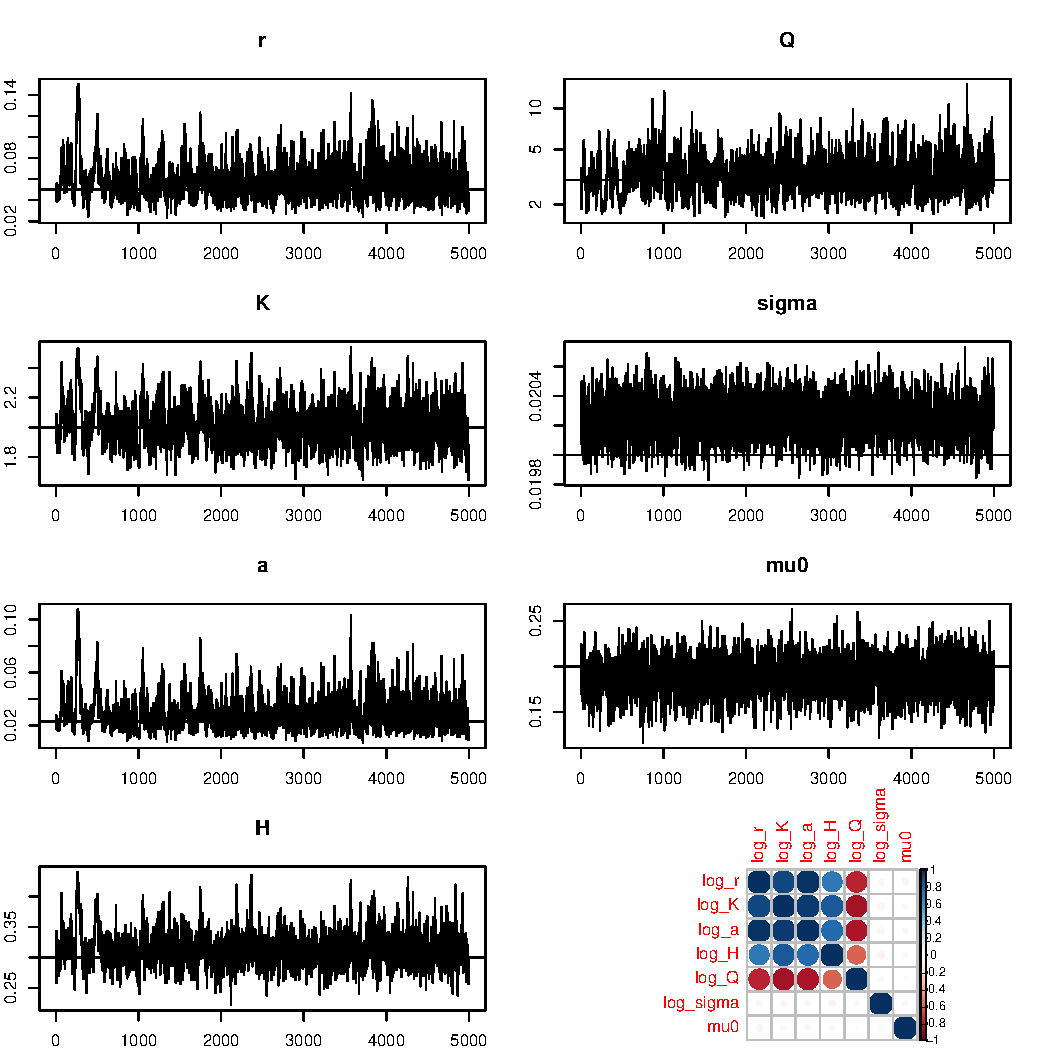
\includegraphics[width=1.00\textwidth]{trace_plots.png}
		\caption{mcmc chains (when all parameters are allowed to vary); note that the parameter values used to generate the data are $r=0.05$, $K=2$, $a=0.023$, $H=0.3$, $q=3$, and $\sigma=0.02$.}
		\label{fig:trace_plots}
	\end{figure}
	%
	\item when we allow a, r, and K to vary, they are highly correlated (bottom right of Figure \ref{fig:trace_plots})
	\item In response to the biased estimators, Lizzie asked Andrew Gelman and Mike Betancourt: ``What diagnostic tools do you recommend for assessing the information contained about a particular parameter, or set of parameters, in the data? What tools do you recommend for designing efficient data collection procedures based on a desire to learn about specific sets of parameters (e.g., how can we determine whether it's better to make observations of trajectories for longer periods of time vs. at higher resolution time scales if we want to learn about $a$)? Under what conditions will the posterior mean/mode be a biased estimator of the ``true'' parameter?''
	\begin{itemize}
		\item Lizzie: both Andrew and Mike honed in on the ``jumps'' in the data (\textcolor{blue}{I don't quite know what these jumps are referring to. Did they think we needed higher temporal resolution?}
		\item Mike suggested following a standard Bayesian workflow to identify what is and is not possible with the model (\textcolor{blue}{Someone stats-y could do this.})
		\item Mike said these types of issues come up a lot in systems where small noise or differences in initial conditions produce wildly different trajectories; one way to demonstrate this is to do proir predictive checks on super tight priors (delta-function priors). See \href{https://betanalpha.github.io/assets/case_studies/principled_bayesian_workflow.html}, step 7. (\textcolor{blue}{Someone stats-y could do this.})
		\item Mike went through the steps we'd need to take: (1) prior predictive checks (2) fit the data from the prior predictive checks (3) check the z-score contraction plot. If the posteriors all collapse to extreme values, your model is non-identifiable. (\textcolor{blue}{Again, someone stats-y could do this.})
		\item \textcolor{blue}{Do we want to do the above things ourselves, or Lizzie also asked if Mike might be willing to join project as co-author and he said sure, if he has time and if not he can recommend good people. Thoughts?}
		\item Andrew: Said we should try to understand the jumps; that's why we replicates are good; otherwise we just have $n=1$ on the jumps; Suggested we get a distribution of timing of jumps and try to understand it. \textcolor{blue}{Would this be similar to a distribution of escape times from the ghost?}
	\end{itemize}
	\item Kai was looking into measuring the amount of learning about parameters that happens (i.e., quantifying the difference between the prior and posterior distribution); Using the the FNN method for KL divergence seemed to be a good approach \textcolor{blue}{Kai, what do you need to go ahead with that?}
\end{itemize}

\subsection{Result from comparing models}

\section{The effect of variance on model dynamics}
\textcolor{blue}{I'm not sure where this should go, but it seems worth thinking about a bit more.}
\begin{itemize}
	\item increasing variance reduces the strength of the ghost attractor (Figure \ref{fig:Effect of variance})
	\item seems to be that the asymmetry of the deterministic curve leads to the positive relationship between higher variance and quicker escapes (Figure \ref{fig:on_why_variance_reduces_the_ghost})
	%\item \hl{plot of ``exit'' times from ghost for different values of sigma (should be skewed with long tails)}
\end{itemize}

\begin{figure}[h]
	\centering
		\includegraphics[width=0.60\textwidth]{Effect_of_variance.png}
	\caption{The effect of variance on the mean trajectory. I plotted the deterministic model core, and then simulated 1000 replicates for 4 different variance levels ($\sigma = 0.005, 0.01, 0.015, 0.02$) and took the mean of each. You can see that even small variance really affects the average trajectory and reduces time spent in the ghost.}
	\label{fig:Effect of variance}
\end{figure}

\begin{figure}[h]
	\centering
		\includegraphics[width=0.60\textwidth]{variance_reducing_ghost.png}
	\caption{State of the art schematic helping me (Jody), at least, understand how symmetric noise reduces time spent in the ghost rather than just adding wiggles around the deterministic core. Henry suggested adding another pair of those red Gaussian curves with even larger (or smaller, depending on what's easier to draw) variance, doing the same A and B experiment and seeing where we wind up. If higher variance leads to quicker escape times, then the average of the two vertical values of A and B should be greater for the higher variance scenario. Higher variance will make it much more likely to reach higher populations, but only slightly more likely to reach lower ones.}
	\label{fig:on_why_variance_reduces_the_ghost}
\end{figure}





%%%%%%%%%%%%%%%%%%%%%%%%%%%%%%%%%%%%%%%%%%%%%%%%%%%%%%%%%%%%%%%%%%%%%%%%%%%%%%%%%%%%%
\section{Discussion}

Stuff we've mentioned:
\begin{itemize}
\item big idea: phenomenological models are bad for forecasting and understanding transient dynamics; mechanistic models may be lauded as a better option to try to get at these things; but even if you have the right mechanisms, there may be tricky estimability issues
	\item Each different single time series effectively looks like a slightly different deterministic version of the model, making inference tricky.
	\item changing the seed for the single trajectory made a big difference in our ability to say anything meaningful about the underlying processes; a possible take home message from Henry: observing a single trajectory is probably not enough to help us learn much about these sophisticated parametric models, but maybe an ensemble of observations is. That general principle is pretty familiar to spatial/temporal statisticians: it's hard to estimate complicated covariance functions for a single observation of a process. They way people overcome the limitation there is typically to just fix or place very informative priors on the hardest to estimate parameters (which also sometimes have the weakest interpretability anyway). Maybe our recommendation for how to address the issue in practice could be similar, with some advice on how to solicit priors or picked fixed values.
	\item The reduction in the strength of the ghost attractor with increasing variance is likely what makes it difficult to get back parameters
	\item Challenges in predicting transient behaviour from real data.
	\item Coming up with new ways to describe phenomenon that perhaps could be better described with another method. For example, for animal movement data, where hidden Markov models are mostly used maybe you should be using dynamical models.
	\item Focusing on phase shifts ... understanding if the behaviour is transient versus phase shift versus observing asymptotic behaviour ... 
	\item If you don't think about transients (by going in with a preformed idea of a system of asymptotic or a mixture model) you can miss important transient behaviour which can be critical prediction.
	\item Are some dynamical models totally intractable statistically?
	\item From all this, get to what you need to know about system (helping improve experiments)  ... If you can observe the system at transient dynamics you can perhaps learn more. 
	\item Transients can arise from inside the system (autonomous) ... so if you cannot find an exogenous factor, maybe it's autonomous to your system
	\item Some other dynamical models with transients (that we dreamed of working on):
		\begin{enumerate}
			\item Linear (matrix model) 
			\item Chaotic
			\item Periodic (fast-slow)
		\end{enumerate}
\end{itemize}

\section*{Issues}

\begin{itemize}
	\item Do we have any hope of detecting a ghost attractor in spite of the biased estimators?
	\item Can we look at the distribution of expected escape times for the posteriors?
	\item As Henry mentioned, it would be nice to have a bit of a positive message to our paper, such as ``in these circumstances, we can say something about transient dynamics'', or something else constructive
	\item from Henry: while the individual parameters may not be strongly identifiable from these types of data, it might be that some other useful quantities are. For instance, how well are we able to resolve the potential function, which encapsulates important information about equilibria and any possible ghosts (Figure fig:posterior_potentials).
	
	%\begin{figure}[h]
		%\centering
			%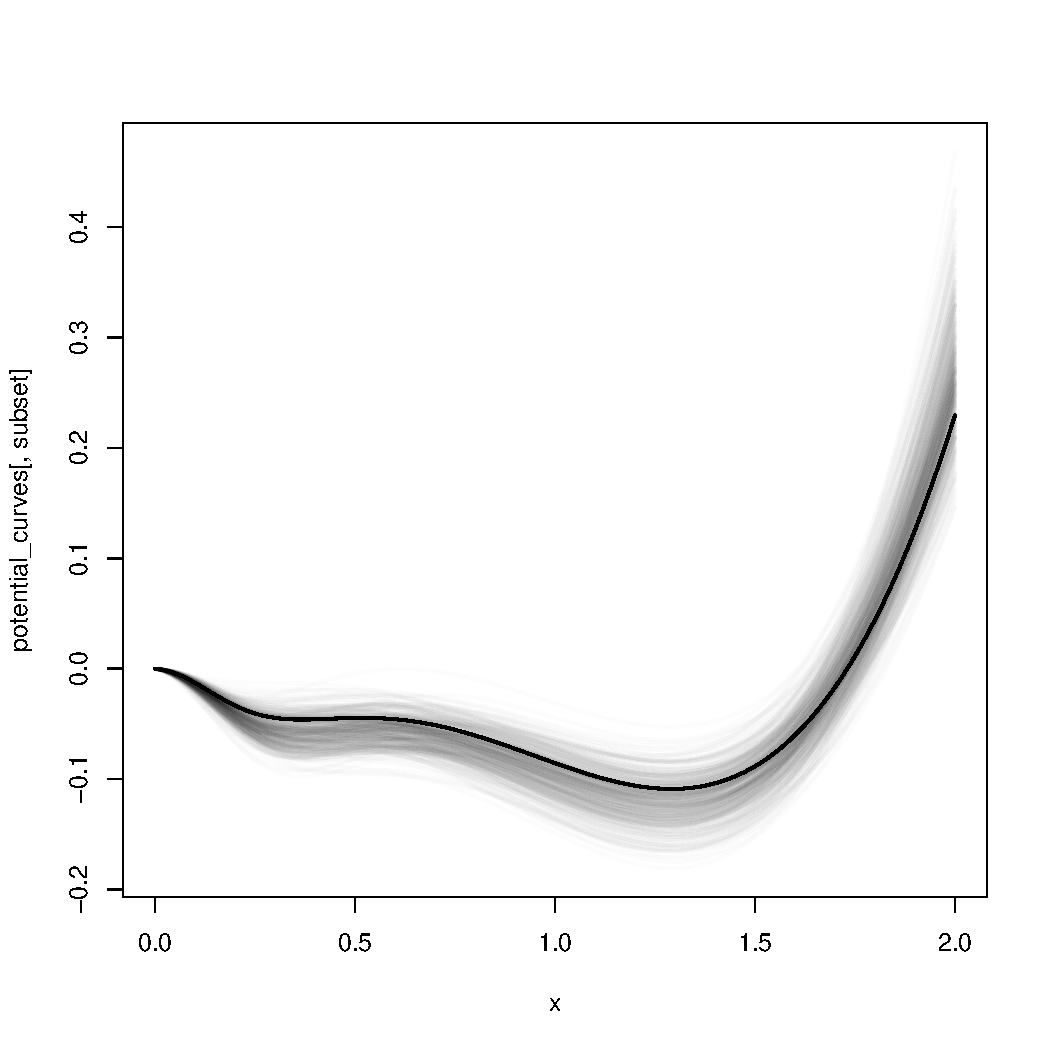
\includegraphics{posterior_potentials.png}
		%\caption{Potential curves drawn from the posteriors in grey; true potential curve in black. Some seem to still suggest the ghost, some suggest 2 stable steady states (i.e., the ``dip'' has dipped too low), and some suggest a steeper curve through the ghost. }
		%\label{fig:posterior_potentials}
	%\end{figure}
	
	\item From when Lizzie talked to Mike: Sometimes with these models it's NOT about needing more time points on a grid, or more points across a grid, it's about needing more points at certain places in the grid. In our case that's probably where the jumps happen (low x to high x).
	\item We can also think about playing with the temporal resolution (e.g., time step of 1/2 instead of 1) or $\sigma$
\end{itemize}

\end{document}